%====================================================================================
\section[Pigou]{Impuesto Pigouviano}
%====================================================================================
\begin{frame}{Impuesto Pigouviano}
	\begin{itemize}
		\item Las externalidades causan ineficiencia debido a la divergencia entre los beneficios (o costos) sociales y privados.
		\item Un impuesto puede usarse para elevar el costo marginal privado
			\begin{itemize}
				\item Esto ayuda a la eficiencia, cuando hay externalidad negativa
			\end{itemize}
		\item Un subsidio puede ser usado para reducir el costo marginal privado
			\begin{itemize}
				\item Esto ayuda a la eficiencia cuando hay una externalidad positiva
			\end{itemize}
		\item Estos impuestos usados para combatir las externalidades son llamados \emph{impuestos Pigouvianos}
	\end{itemize}
\end{frame}
%------------------------------------------------
\begin{frame}{Impuesto Pigouviano}
	Volviendo al ejemplo:
	\begin{itemize}
		\item Supongamos que se establece un impuesto de t unidades monetarias por unidad de contaminación.
		\item El problema de maximización de beneficio de la acería será:
			$$\M \limits_{s,x} \pi_s = p_ss-c_s(s,x)-tx$$
		\item por CPO:
				$$
				\begin{array}{rcr}
					\frac{\partial \pi}{\partial s} = 0 \Leftrightarrow p_s - \frac{\partial c_s}{\partial s} =0 &{}& \frac{\partial \pi}{\partial x} = 0 \Leftrightarrow - \frac{\partial c_s}{\partial x} - t = 0\\[0.3cm]
					p_s = \frac{\partial c_s}{\partial s} &{}& t = - \frac{\partial c_s}{\partial x}
				\end{array}
				$$
		\item En consecuencia, para llegar  a la condición de eficiencia debe cumplirse que:
		$$t = \frac{\partial c_f}{\partial x}$$
	\end{itemize}
\end{frame}
%------------------------------------------------
\begin{frame}{Impuesto Pigouviano: Gráficamente}
	\begin{center}
		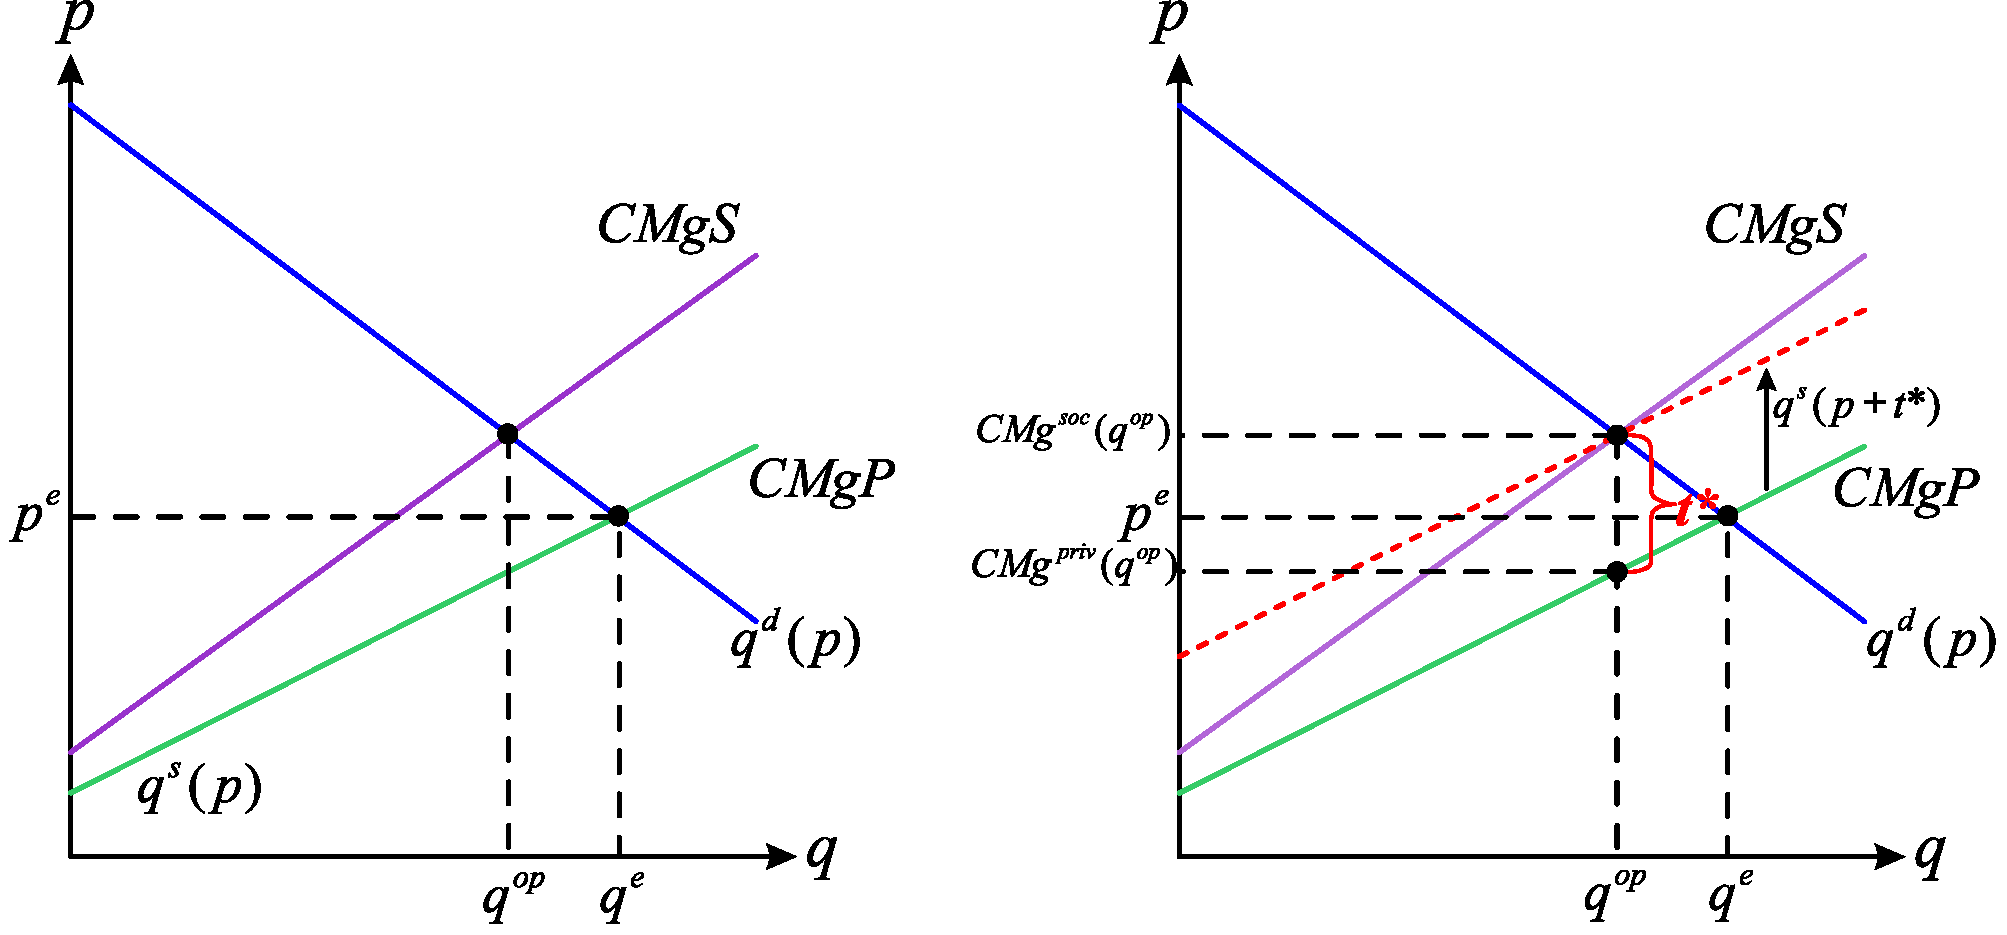
\includegraphics[width = 1\linewidth]{figures/impuestos.pdf}
	\end{center}
\end{frame}
%------------------------------------------------
\begin{frame}{Impuesto Pigouviano}
	\begin{itemize}
		\item El impuesto Pigouviano parece ser una solución simple
				\begin{itemize}
					\item El impuesto pagado = daño marginal
					\item El subsidio recibido = beneficio marginal
				\end{itemize}
		\item Pero hay limitaciones
				\begin{itemize}
					\item Los impuestos pueden necesitar ser diferenciados entre consumidores, empresas y bienes.
					\item Sin diferenciación suficiente, la externalidad sería corregida sólo parcialmente
					\item La intervención puede ser también requerida en los mercados de bienes relacionados
				\end{itemize}
		\item El impuesto debe ser visto como poner un precio a la externalidad.
	\end{itemize}
\end{frame}